%% 
%% Copyright 2019-2020 Elsevier Ltd
%% 
%% This file is part of the 'CAS Bundle'.
%% --------------------------------------
%% 
%% It may be distributed under the conditions of the LaTeX Project Public
%% License, either version 1.2 of this license or (at your option) any
%% later version.  The latest version of this license is in
%%    http://www.latex-project.org/lppl.txt
%% and version 1.2 or later is part of all distributions of LaTeX
%% version 1999/12/01 or later.
%% 
%% The list of all files belonging to the 'CAS Bundle' is
%% given in the file `manifest.txt'.
%% 
%% Template article for cas-dc documentclass for 
%% double column output.

%\documentclass[a4paper,fleqn,longmktitle]{cas-dc}
%\documentclass[5p,times]{cas-dc}
%\documentclass[5p,times]{elsarticle}
\documentclass[5p,times]{elsarticle}


\usepackage{amsmath} % For mathematical expressions
\usepackage{amssymb} % For mathematical symbols
\usepackage{algorithm} % For pseudocode
\usepackage{algpseudocode} % For pseudocode

%\usepackage[numbers]{natbib}
%\usepackage[authoryear]{natbib}
%\usepackage[authoryear,longnamesfirst]{natbib}
%cai o ben duoi bo orcid(s)
%\let\printorcid\relax
\usepackage{amsmath}
\usepackage{amssymb}
\usepackage{amsfonts}
\usepackage{multirow}
\usepackage{longtable}
\usepackage{caption}
\usepackage{subcaption}
\usepackage{pifont}
\usepackage{array}
\usepackage{url}
\usepackage{xcolor}
\usepackage[colorlinks=true,allcolors=white]{hyperref}
\usepackage{makecell}
\usepackage{booktabs} 
\usepackage{stfloats}


\usepackage{minted}

\newcolumntype{P}[1]{>{\centering\arraybackslash}p{#1}}

\usepackage[switch]{lineno}


% %%%Author definitions
% \def\tsc#1{\csdef{#1}{\textsc{\lowercase{#1}}\xspace}}
% \tsc{WGM}
% \tsc{QE}
% \tsc{EP}
% \tsc{PMS}
% \tsc{BEC}
% \tsc{DE}
% %%%

% Uncomment and use as if needed
%\newtheorem{theorem}{Theorem}
%\newtheorem{lemma}[theorem]{Lemma}
%\newdefinition{rmk}{Remark}
%\newproof{pf}{Proof}
%\newproof{pot}{Proof of Theorem \ref{thm}}

\begin{document}

\let\WriteBookmarks\relax
\def\floatpagepagefraction{1}
\def\textpagefraction{.001}

% Short title
%\shorttitle{Raijū: Reinforcement Learning-Guided Post-Exploitation for Automating Security Assessment of Network Systems}

% Short author
%\shortauthors{Van-Hau Pham et~al.}

% Main title of the paper
\title{tieu de bai bao RAG provacy FL.... }                      
% Title footnote mark
% eg: \tnotemark[1]
%\tnotemark[1,2]

% Title footnote 1.
% eg: \tnotetext[1]{Title footnote text}
% \tnotetext[<tnote number>]{<tnote text>} 
%\tnotetext[1]{This document is the results of the research
%   project funded by the National Science Foundation.}

%\tnotetext[2]{The second title footnote which is a longer text matter
%   to fill through the whole text width and overflow into
%   another line in the footnotes area of the first page.}


% First author
%
% Options: Use if required
% eg: \author[1,3]{Author Name}[type=editor,
%       style=chinese,
%       auid=000,
%       bioid=1,
%       prefix=Sir,
%       orcid=0000-0002-1489-2826,
%       facebook=<facebook id>,
%       twitter=<twitter id>,
%       linkedin=<linkedin id>,
%       gplus=<gplus id>]


\affiliation[1]{organization={Information Security Lab, University of Information Technology},
    city={Ho Chi Minh City},
    country={Vietnam}}
\affiliation[2]{organization={Vietnam National University Ho Chi Minh City},
    city={Ho Chi Minh City},
    country={Vietnam}}

\author[1,2]{Nguyen Hoang Duy}%\fnref{fn2}}
\ead{22520329@gm.uit.edu.vn}

\author[1,2]{Le Vu Ca}%\fnref{fn2}}
\ead{22520140@gm.uit.edu.vn}

\author[1,2]{Van-Hau Pham}%\fnref{fn6}}
\ead{haupv@uit.edu.vn}

\author[1,2]{Phan The Duy\corref{cor1}}
\ead{duypt@uit.edu.vn}
\cortext[cor1]{Corresponding author}


% \cortext[cor1]{Corresponding author}
% \fntext[fn1]{}
% \fntext[fn2]{}
% \fntext[fn3]{}
% \fntext[fn4]{}
% \fntext[fn5]{}
% \fntext[fn6]{}
% % 5 author
% \author[1,2]{Van-Hau Pham}[%
%    %role=Co-ordinator,
%    %suffix=PhD,
%    ]
% % 6 author
% \author[1,2]{Nguyen Tan Cam}[%
%    style=editor,   
%    role=Corresponding author,
%    orcid=0000-0002-3909-7650,
%    %suffix=PhD,
%    ]
   
% \fnmark[*]
% \ead{camnt@uit.edu.vn}
% \ead[URL]{www.uit.edu.vn}

%\credit{Data curation, Writing - Original draft preparation}

% Address/affiliation
%\affiliation[2]{organization={Sayahna Foundation},
    % addressline={}, 
 %   city={Jagathy},
    % citysep={}, % Uncomment if no comma needed between city and postcode
 %   postcode={695014}, 
  %  state={Trivandrum},
  % country={India}}

% Fourth author
%\author%
%[1,3]
%{Rishi T.}
%\cormark[2]
%\fnmark[1,3]
%\ead{rishi@stmdocs.in}
%\ead[URL]{www.stmdocs.in}

%\affiliation[3]{organization={STM Document Engineering Pvt Ltd.},
%    addressline={Mepukada}, 
%    city={Malayinkil},
    % citysep={}, % Uncomment if no comma needed between city and postcode
 %   postcode={695571}, 
 %   state={Trivandrum},
 %   country={India}}

% Corresponding author text
%\cortext[cor1]{Corresponding author}
%\cortext[cor2]{Principal corresponding author}

% Footnote text
%\fntext[fn1]{This is the first author footnote. but is common to third
%  author as well.}
%\fntext[fn2]{Another author footnote, this is a very long footnote and
%  it should be a really long footnote. But this footnote is not yet
%  sufficiently long enough to make two lines of footnote text.}

% For a title note without a number/mark
%\nonumnote{This note has no numbers. In this work we demonstrate $a_b$
%  the formation Y\_1 of a new type of polariton on the interface
%  between a cuprous oxide slab and a polystyrene micro-sphere placed
%  on the slab.
%  }

% Here goes the abstract
\begin{abstract}
..... tom tat bai bao....
 

 
\end{abstract}


\begin{keyword}
Federated Learning \sep Intrusion Detection System \sep Poisoning Attack \sep Non-IID  \sep Proactive Defense \sep Probe Vector
\end{keyword}


% Keywords
% Each keyword is seperated by \sep


% Use if graphical abstract is present
% \begin{graphicalabstract}
% \includegraphics{figs/grabs.pdf}
% \end{graphicalabstract}

\maketitle

\section{Introduction} \label{sec_introduction}
...

In summary, our main contributions are as follows:
\begin{itemize}
\item bbbb.
\item bbbbbb
\item bbbbmm
\item vvv.
\end{itemize}

The remainder of this article is organized as follows. Section \ref{sect_relatedworks} presents the related work. Section \ref{sect:methodology} describes the proposed methodology in detail. Next, Section \ref{sec_experiment} presents the dataset and experimental setup, followed by Section \ref{sect_results} with performance evaluation and analysis. We discuss threats to validity in Section \ref{sect_threats_tovalidity}. Finally, Section \ref{sec_conclusion} concludes the article and outlines future directions.

\begin{table*}[ht]
\centering
\caption{Comparison of Federated Learning Defense Mechanisms (Simplified)}
\label{tab:compare}
\small
\begin{tabular}{l l l c c c c c}
\toprule
\textbf{Method} & \textbf{Defense Type} & \textbf{Attack Type} & \textbf{Clean Data} & 
\textbf{Non-IID} & \textbf{Overhead} & \textbf{Temporal} & \textbf{Multi-layer} \\
\midrule
FedAMM \cite{11175562}     & Robust + Clustering & Backdoor (majority) & No  & High   & High   & No  & Yes \\
TMT-FL \cite{lu2025tmtfl}    & Cryptographic (ZKP) & Data/model poison   & No  & Low    & High   & Yes & Yes \\
RECESS \cite{yan2025recess}     & Proactive + Robust  & Model poison (MPA)  & No  & Medium & Medium & Yes & Part \\
DPAD \cite{BASAK2025109893}       & Audit-based         & Data poisoning      & Yes & Low    & High   & No  & No \\
MSGuard \cite{yang2025msguard}    & Multi-strategy      & Sign, ALIE, MinMax  & No  & Medium & High   & No  & No \\
FLGuardian \cite{zhou2025flguardian} & Layer detection     & Backdoor (layer)    & No  & Medium & Medium & Yes & Yes \\
FedCleanse \cite{HUANG2025114494} & Post-agg, Neuron    & Backdoor (replace)  & No  & High   & Low    & Yes & Yes \\
FedMP \cite{ZHAO2025110990}      & Multi-pronged       & Byzantine (SF,LIE)  & No  & High   & Medium & No  & No \\
FLANDERS \cite{11164345}   & Pre-agg + Time-ser  & Untargeted poison   & No  & High   & High   & Yes & Part \\
UDFed \cite{Deng2025UDFedAU}     & Hybrid Universal    & Noise, LIE, Backdoor& No  & Medium & Low    & Yes & Yes \\

Fed-LSAE \cite{FedLSAE} & Latent-space (Pre-agg) & Label-flip, GAN, Weight-scale & No & High & Low & No & Part \\

\textbf{P4P (ours)} & Proactive + Multi & Universal (Byz+BD) & No & High & Low & Yes & Yes \\
\bottomrule
\end{tabular}
\end{table*}


 
\section{Related Work} \label{sect_relatedworks}

\subsection{Federated Learning and Intrusion Detection Systems (IDS)}
Federated Learning (FL) has been widely adopted in security-sensitive applications, particularly for building Intrusion Detection Systems (IDS) in distributed IoT and edge environments. By allowing multiple clients to collaboratively train a global model without sharing raw data, FL preserves privacy while leveraging diverse datasets \cite{kairouz2021advances,Nguyen2022}. However, the same decentralization that makes FL attractive also increases its vulnerability to adversarial manipulation. For IDS, where the correctness of anomaly detection is crucial, poisoned updates from a few compromised clients can significantly degrade detection accuracy or even implant backdoors for stealthy intrusions \cite{Liu2020}. Recent advances, such as Fed-LSAE \cite{FedLSAE}, highlight a shift toward latent-space inspection for FL-based IDS, leveraging feature representations instead of raw parameters to enhance robustness against internal poisoning.


\subsection{Model Poisoning Attack}
Among the threats to FL, model poisoning attacks are particularly dangerous. Unlike data poisoning, which corrupts training inputs, model poisoning directly manipulates gradients or weight updates. Attack vectors include sign-flipping, Gaussian perturbations, and label-flipping, as well as more sophisticated strategies such as Little is Enough (LIE), backdoors, and stealthy scaling attacks \cite{fang2020local,Bhagoji2019,baruch2019}. These methods enable adversaries to either degrade global accuracy (untargeted Byzantine attacks) or inject malicious behavior into the global model (targeted backdoors). In Non-IID settings typical of IDS deployments, benign clients naturally produce divergent updates, making it even harder to distinguish between malicious and honest contributions \cite{Shejwalkar2021}.


\subsection{Secured Aggregation and Defense Mechanisms}
To counter poisoning, a broad range of defenses have been proposed. Passive approaches, such as FedMP \cite{ZHAO2025110990}, FL-Guardian \cite{11003999}, DPAD \cite{BASAK2025109893}, and MSGuard \cite{10942405}, rely on anomaly detection or clustering of submitted updates. While effective in controlled settings, they incur high computational overhead and often assume majority honesty, which is fragile under Non-IID distributions. Proactive defenses, such as RECESS \cite{10851419}, introduce active probes (e.g., gradient traps) but remain sensitive to adaptive attackers. Cryptographic methods, including TMT-FL \cite{10812212}, guarantee data integrity through zero-knowledge proofs or blockchain auditing, yet their costs are prohibitive and they do not directly detect semantic poisoning. More recent multi-layer defenses (e.g., FedAMM \cite{11175562}, FedCleanse \cite{HUANG2025114494}, UDFed \cite{Sun2023}, Time-Series Defense \cite{Li2025}) combine multiple signals such as reputation, gradient decomposition, or temporal anomaly detection. In parallel, Fed-LSAE \cite{FedLSAE} introduces a lightweight latent-space inspection defense that filters clients via penultimate-layer representations, Autoencoder compression, and RBF-CKA clustering to exclude malicious participants, yet it assumes a minority of attackers and a fixed configuration. While these strategies improve robustness, they remain limited by scalability, high computational costs, or lack of proactive verification. 


\begin{figure*}[ht]
  \centering
  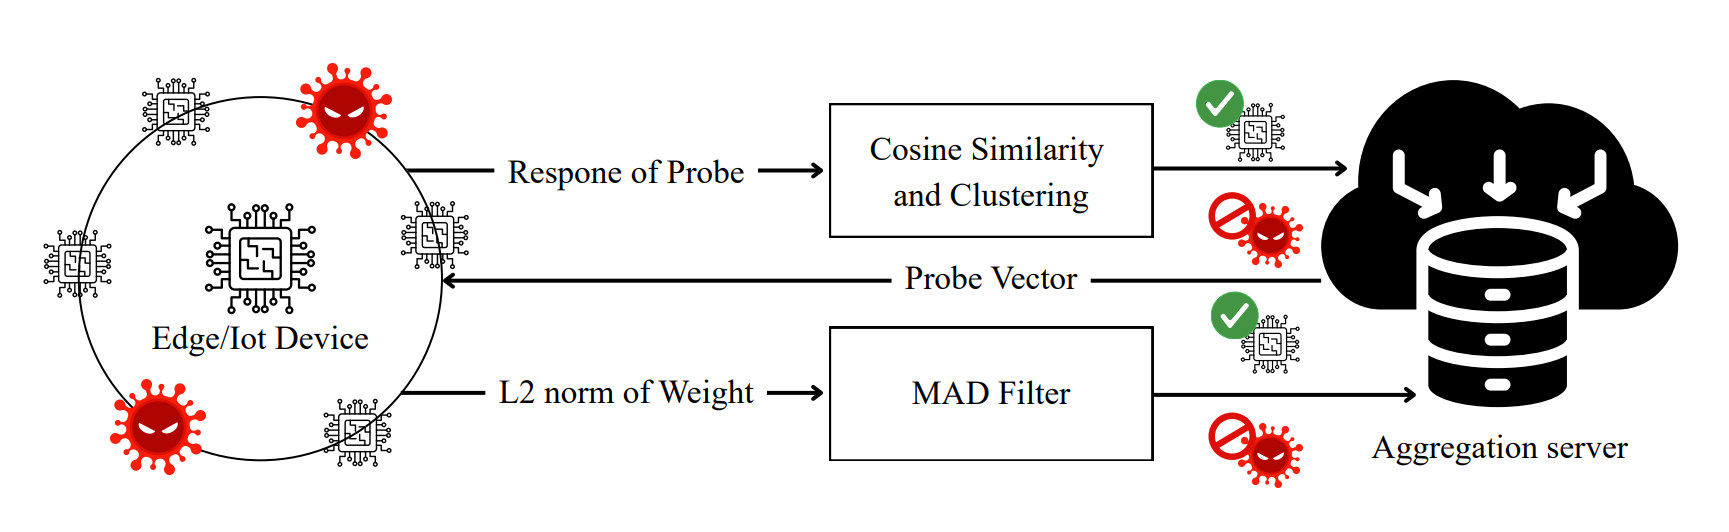
\includegraphics[width=1\linewidth]{images/overview.png}
  \caption{Overview of the proposed Defense Mechanism.}
  \label{fig:framework}
\end{figure*}

\subsection{Non-IID Issues}
A fundamental limitation across most defenses is the Non-IID nature of federated datasets. IDS clients often monitor highly heterogeneous traffic patterns, leading to natural divergence of updates. Defenses that assume benign clients converge toward a majority direction (e.g., MSGuard, FL-Guardian) misclassify honest but divergent clients as adversaries, increasing false positives. Conversely, adaptive attackers can exploit this heterogeneity to camouflage poisoned updates \cite{Shejwalkar2021,Fu2022}. Furthermore, most defenses evaluate updates independently at each round, without considering temporal consistency, leaving them vulnerable to stealthy or slow poisoning \cite{fang2020local}. Fed-LSAE \cite{FedLSAE} alleviates some Non-IID variance through Autoencoder-compressed latent representations but performs round-wise filtering without temporal adaptation.


In light of these challenges, a new defense mechanism must (i) remain lightweight for deployment in edge-based IDS, (ii) operate without clean validation datasets, (iii) adapt to Non-IID environments, and (iv) incorporate temporal analysis to detect stealthy adversaries. Our proposed P4P framework directly addresses these requirements by leveraging probe vectors and temporal chaining in a proactive multi-layer design.

\subsection{Pipeline Overview}

As summarized in Table~\ref{tab:compare}, existing defenses either incur
high computational costs, rely on clean validation data, or fail to handle
Non-IID scenarios effectively. In contrast, our proposed P4P framework
achieves low overhead, strong Non-IID robustness, and temporal resilience,
making it a lightweight yet proactive multi-layer defense.





\section{Methodology} \label{sect:methodology}

\subsection{Framework Overview}
The core objective of our P4P framework, is to provide a proactive, lightweight, and multi-layer defense against poisoning attacks in FL. 
Existing defense strategies either rely on static aggregation rules or complex cryptographic primitives. 
Static rules (e.g., Krum, Trimmed Mean) treat client updates independently at each round and are vulnerable to collusion or stealthy poisoning, while cryptographic approaches (e.g., secure multiparty computation or blockchain-based logging) incur prohibitive overhead and still do not directly address model update manipulation. 
To overcome these limitations, we design P4P with three guiding principles: 


Proactivity: Instead of passively observing updates, the server actively queries clients using probe vectors derived from the global trajectory. 

Temporal awareness: Malicious behaviors often manifest gradually or intermittently. By chaining probe vectors across rounds, the server leverages historical consistency to expose stealthy strategies.

Lightweight robustness: Defense mechanisms must be practical in large-scale deployments. P4P transforms high-dimensional updates into low-dimensional probe responses, enabling efficient anomaly detection with minimal cost.


Figure~\ref{fig:framework} illustrates the overall architecture of P4P. At each round, the server constructs a probe vector, broadcasts it to clients, collects probe responses and updates, applies multi-layer detection, and finally aggregates only trusted contributions into the global model. 

\subsection{Probe Vector Construction}

One of the central novelties of P4P lies in the construction and use of \textit{probe vectors}. 
Rather than assuming that the majority of client updates are benign, which may not hold under collusion, the server instead relies on its own historical trajectory as a stable reference. 

Given the global parameters $W_t \in \mathbb{R}^d$ at round $t$, the probe vector is defined as:

\begin{equation}
    v_t = W_t - W_{t-1}.
\end{equation}

This formulation captures the \textit{incremental direction} of model evolution between two consecutive rounds. 
It has two desirable properties: (1) it encodes temporal history, meaning that adversaries cannot easily alter it without consistently corrupting many rounds; (2) it is model-dependent but data-agnostic, requiring no access to raw data or trusted clean datasets. 

Alternative approaches, such as computing references from small server-side datasets, are either unrealistic (clean data may not exist) or introduce bias (server data not representative of client distributions). 
By contrast, the probe vector leverages only information already available to the server.

As shown in Figure \ref{fig:pipeline}, the probe vector provides a global reference that reduces Non-IID bias. While benign clients align with the probe, suspicious clients deviate due to Non-IID heterogeneity, and malicious clients cluster in the opposite direction, enabling clustering-based separation.

\begin{figure}[ht]
  \centering
  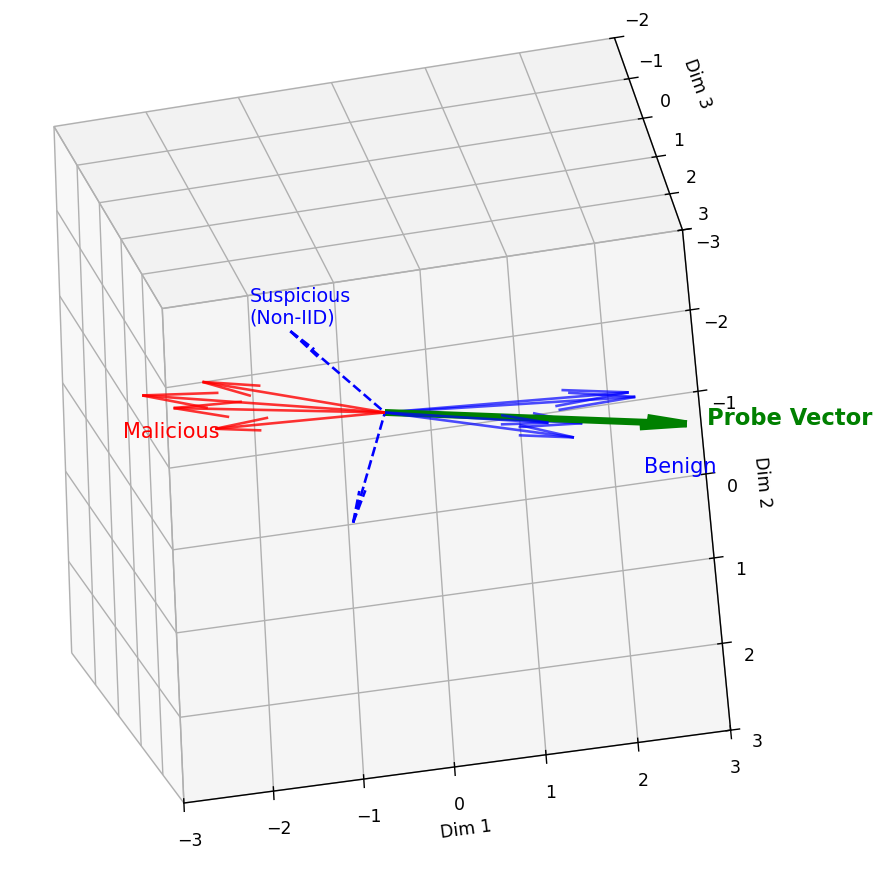
\includegraphics[width=1\linewidth]{Screenshot 2025-09-30 145946.png}
  \caption{Caculate consines similarity between Clients and Probe Vector then Clustering}
  \label{fig:pipeline}
\end{figure}

\subsection{Client Probe Response}

Upon receiving $v_t$, each client $C_i$ computes its \textit{probe response} $r_i^t$ by measuring the cosine similarity between its local update $\Delta W_i^t$ and $v_t$:

\begin{equation}
    r_i^t = \frac{\langle \Delta W_i^t, v_t \rangle}{\|\Delta W_i^t\|_2 \cdot \|v_t\|_2}.
\end{equation}

This scalar response compresses high-dimensional updates into a single interpretable score. 
High values ($r_i^t \approx 1$) indicate alignment with the global trajectory, as expected from benign clients. 
Low or negative values indicate divergence or sign flipping, typical of malicious updates. 

This transformation is crucial for scalability: a model with millions of parameters can be reduced to a one-dimensional similarity measure per client, enabling lightweight clustering and anomaly detection. 
Moreover, since all clients are evaluated against the same reference $v_t$, non-IID heterogeneity is normalized, reducing false positives.

\subsection{Multi-layer Defense Mechanism}
To ensure robustness, P4P does not rely solely on probe responses but integrates them into a multi-layer pipeline.

\subsubsection{L2-norm Filtering}
\begin{figure}[ht]
  \centering
  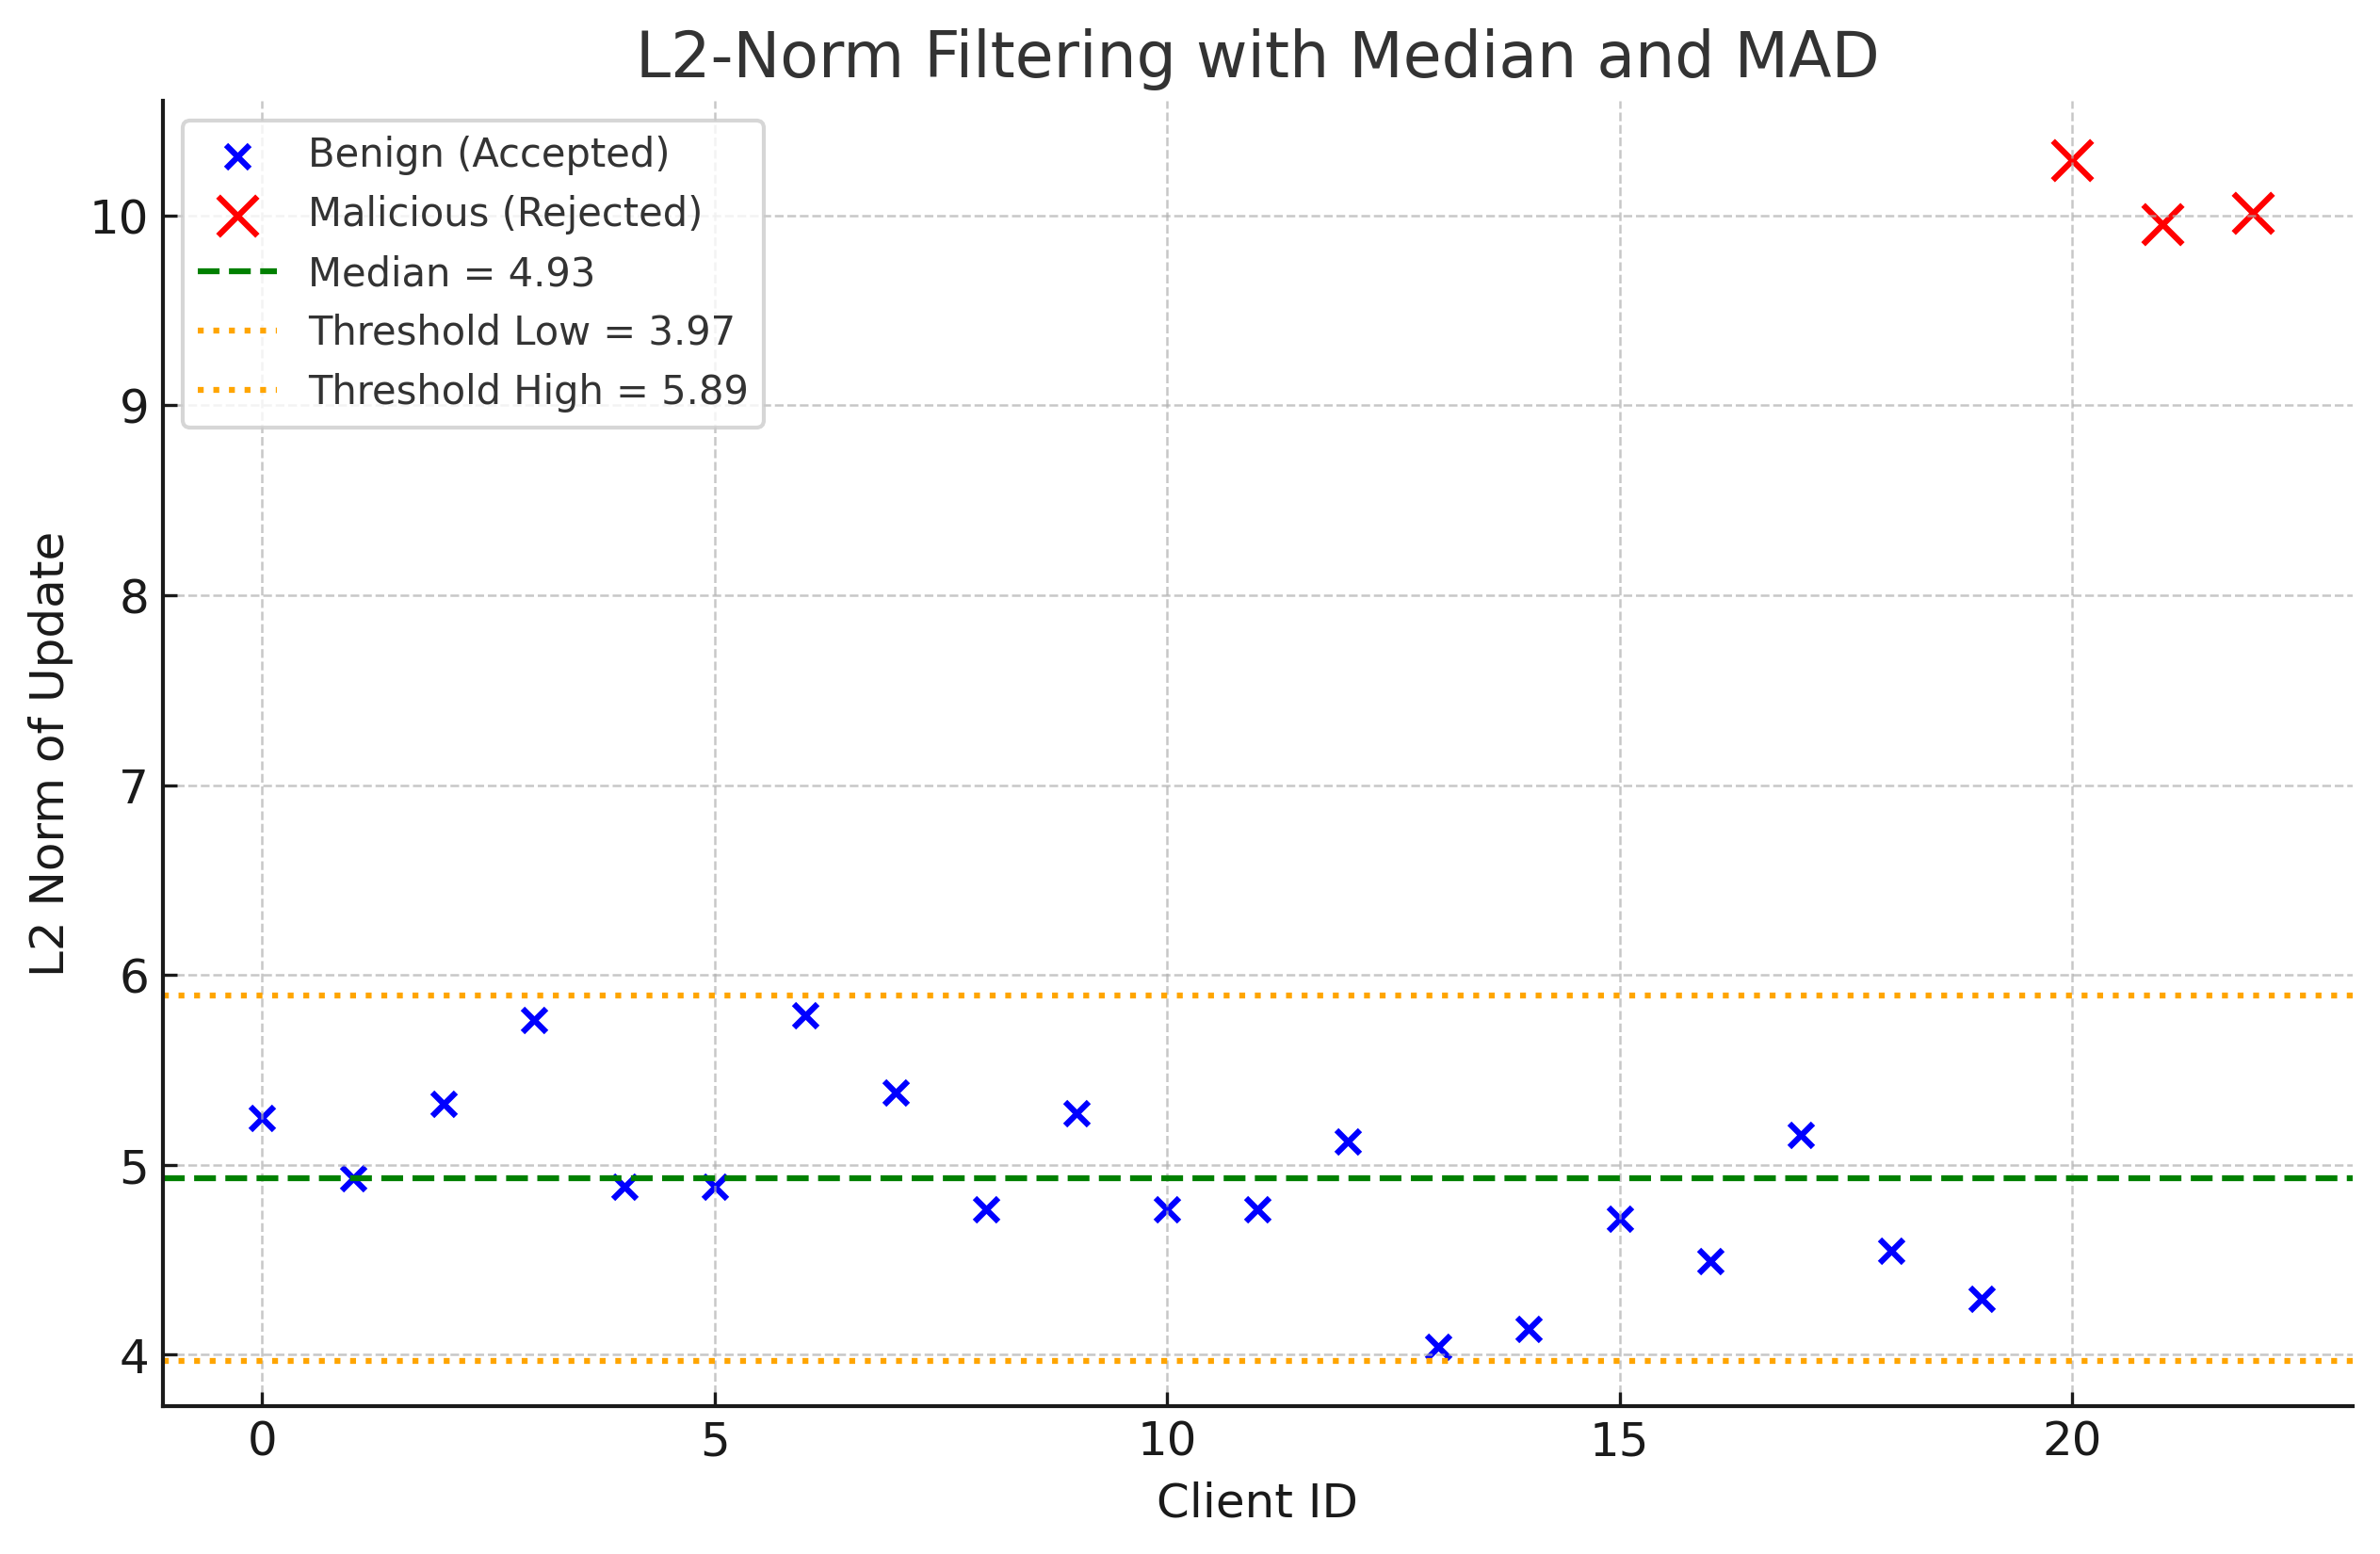
\includegraphics[width=1\linewidth]{l2_norm_filtering.png}
  \caption{Graph construction and representation process of heterogeneous graphs.}
  \label{fig:MADFilter}
\end{figure}
We first evaluate the scale of each update by its L2 norm:

\begin{equation}
    \|\Delta W_i^t\|_2 = \sqrt{\sum_{j=1}^d (\Delta W_{i,j}^t)^2}.
\end{equation}

Malicious clients often inject updates with abnormally large magnitudes to dominate aggregation. 

To robustly filter such outliers, we apply Median Absolute Deviation (MAD):

\begin{equation}
    \text{MAD} = \text{median} \left( \big| \|\Delta W_i^t\|_2 - \text{median}(\|\Delta W^t\|_2) \big| \right).
\end{equation}

Updates exceeding a threshold (e.g., $3 \times$ MAD) are temporarily flagged. 

This step prevents simple scaling attacks. As show in Figure~\ref{fig:MADFilter}, this step prevents attacks base on scaling weight.


\subsubsection{Probe-based Anomaly Detection}
Next, the probe responses $\{r_i^t\}$ are analyzed using an ensemble of detectors:

\begin{itemize}
    \item \textbf{KMeans clustering}: partitions responses into two groups; minority clusters are suspect.
    \item \textbf{DBSCAN}: detects density-based anomalies; isolated clients (label $=-1$) are suspect.
    \item \textbf{Isolation Forest}: identifies statistical outliers; responses with low isolation scores are suspect.
\end{itemize}

% =============================
% Algorithm 2: Probe-based Anomaly Detection
% =============================
\begin{algorithm}[H]
\caption{Probe-based Anomaly Detection (Ensemble Voting)}
\KwIn{Probe responses $\{r_i^t\}_{i=1}^N$, client IDs $\{C_i\}$}
\KwOut{Suspicious client set $\mathcal{S}_{anom}$}

Initialize votes[$i$] $\gets 0$ for all clients\;

\textbf{Step 1: KMeans Clustering}\;
Cluster $\{r_i^t\}$ into 2 groups\;
Assign vote[$i$]++ if client $i$ belongs to minority cluster\;

\textbf{Step 2: DBSCAN}\;
Run DBSCAN on $\{r_i^t\}$\;
Assign vote[$i$]++ if client $i$ is labeled as noise ($-1$)\;

\textbf{Step 3: Isolation Forest}\;
Fit Isolation Forest on $\{r_i^t\}$\;
Assign vote[$i$]++ if client $i$ is predicted as outlier\;

$\mathcal{S}_{anom} \gets \{ i \mid \text{votes}[i] \geq 2 \}$\;

\Return $\mathcal{S}_{anom}$\;
\end{algorithm}
Each detector provides a vote, and a client is considered suspicious if flagged by at least two. 
This ensemble approach increases robustness against adaptive attacks designed to bypass a single detector.



\subsubsection{Temporal Suspicion Scoring}
To address intermittent poisoning and reduce false positives, we introduce a suspicion score $s_i^t$:

\begin{equation}
    s_i^t = \max(0, s_i^{t-1} + \delta_i^t - \gamma),
\end{equation}

where $\delta_i^t=1$ if client $C_i$ is flagged at round $t$ and $0$ otherwise, and $\gamma$ is a decay factor allowing benign clients to recover over time. 
If $s_i^t > \theta$, the client is permanently removed. 
% =============================
% Algorithm 3: Temporal Suspicion Scoring
% =============================
\begin{algorithm}[H]
\caption{Temporal Suspicion Scoring}
\KwIn{Previous scores $s_i^{t-1}$, suspicious set $\mathcal{S}_{anom}$, decay $\gamma$, threshold $\theta$}
\KwOut{Updated scores $s_i^t$, permanently removed clients $\mathcal{R}$}

$\mathcal{R} \gets \emptyset$\;

\ForEach{client $i$}{
    \eIf{$i \in \mathcal{S}_{anom}$}{
        $s_i^t \gets s_i^{t-1} + 1$\;
    }{
        $s_i^t \gets \max(0, s_i^{t-1} - \gamma)$\;
    }
    \If{$s_i^t > \theta$}{
        add $i$ to $\mathcal{R}$\;
    }
}
\Return $(s_i^t, \mathcal{R})$\;
\end{algorithm}

This mechanism leverages temporal history, ensuring that malicious behavior accumulating over rounds is detected, while benign clients with occasional deviations are not unfairly penalized.
% ===================================
% Algorithm 3: Server-side Detection + Aggregation
% ===================================
\begin{algorithm}[H]
\caption{ServerProcedure($W_t, \{\Delta W_i^t, r_i^t\}, \{s_i\}$)}
\KwIn{Global model $W_t$, client updates $\{\Delta W_i^t\}$, probe responses $\{r_i^t\}$, suspicion scores $\{s_i\}$}
\KwOut{Updated global model $W_{t+1}$}

\tcp{L2-norm filtering}
Compute $l_i = \|\Delta W_i^t\|_2$\;
$m \gets \text{median}(\{l_i\})$, \quad $\text{MAD} \gets \text{median}(|l_i - m|)$\;
$\mathcal{S}_{norm} \gets \{ i : |l_i - m| \leq \tau \cdot \text{MAD} \}$\;

\tcp{Probe-based ensemble anomaly detection}
Initialize votes[$i$] $\gets 0$\;
Run KMeans, DBSCAN, Isolation Forest on $\{r_i^t\}$\;
Increment votes[$i$] for outliers\;
$\mathcal{S}_{anom} \gets \{ i : \text{votes}[i] \geq 2 \}$\;

\tcp{Temporal suspicion scoring}
\ForEach{$i \in \mathcal{S}_{norm}$}{
    \eIf{$i \in \mathcal{S}_{anom}$}{
        $s_i \gets s_i + \delta$\;
    }{
        $s_i \gets \max(0, s_i - \gamma)$\;
    }
    \If{$s_i > \theta$}{
        mark client $i$ as permanently malicious\;
    }
}

\tcp{Aggregation from trusted clients}
$\mathcal{S}_{trust} \gets \mathcal{S}_{norm} \setminus \mathcal{R}$\;
$W_{t+1} \gets W_t + \eta \cdot \frac{\sum_{i \in \mathcal{S}_{trust}} \Delta W_i^t}{|\mathcal{S}_{trust}|}$\;

\Return $W_{t+1}$\;
\end{algorithm}
\subsection{Robust Aggregation}
Finally, trusted updates are aggregated to update the global model. 
We adopt a weighted FedAvg scheme:

\begin{equation}
    W_{t+1} = W_t + \eta \cdot \frac{\sum_{i=1}^N \omega_i^t \Delta W_i^t}{\sum_{i=1}^N \omega_i^t},
\end{equation}

where $\omega_i^t \in \{0,1\}$ indicates whether client $C_i$ is trusted at round $t$, and $\eta$ is the global learning rate. 
\usepackage[ruled,vlined]{algorithm2e}



By integrating multiple layers of defense before aggregation, P4P minimizes the influence of malicious updates and maintains the integrity of the global model.

\subsection{Workflow Summary}
The complete P4P workflow can be summarized as follows:

\begin{enumerate}
    \item \textbf{Probe vector construction:} The server computes $v_t = W_t - W_{t-1}$ from consecutive global models.
    \item \textbf{Client probing:} Each client computes $r_i^t$ by measuring cosine similarity between $\Delta W_i^t$ and $v_t$, and returns both $\Delta W_i^t$ and $r_i^t$.
    \item \textbf{Multi-layer detection:} The server applies L2-norm filtering, ensemble anomaly detection on $\{r_i^t\}$, and temporal suspicion scoring.
    \item \textbf{Robust aggregation:} Updates from trusted clients are aggregated to form $W_{t+1}$.
\end{enumerate}
\section{Implementation and Experiment Settings} \label{sec_experiment}
This section presents a comprehensive evaluation of our proposed dual-branch framework. We organize the experiments around three research questions (RQs), describe the datasets and experimental setup, and then report results on in-dataset, cross-dataset, and adversarial robustness evaluations. Our goal is to rigorously assess accuracy, generalization, and resilience. 

\begin{table*}[ht]
\centering
\caption{Summary of datasets used in the experiments.}
\label{tab:dataset}
\begin{tabular}{lccccc}
\toprule
\textbf{Dataset} & \textbf{Year} & \textbf{Samples} & \textbf{Features} & \textbf{Classes} & \textbf{Used} \\
\midrule
IoTDIAD & 2023 & $\sim$1.2M & 35 & 9 (1 benign + 8 attacks) & 180k \\
ACI IoT & 2023 & $\sim$25M & 42 & 16 (1 benign + 15 attacks) & 320k \\
\bottomrule
\end{tabular}
\end{table*}

\subsection{Research Questions}
To evaluate the performance of our approach, we define the following research questions:
\begin{itemize}
    \item \textbf{RQ1: Defense Effectiveness.} Does P4P maintain higher accuracy and achieve a lower Attack Success Rate (ASR) than existing defense methods under Byzantine and Backdoor attack scenarios?
    
    \item \textbf{RQ2: Non-IID Robustness.} Can P4P accurately detect malicious updates without confusing them with Non-IID induced drifts, and perform better than baseline approaches?
    
    \item \textbf{RQ3: Component Contribution.} What is the contribution of each individual component of the P4P framework (i.e., Probe Vector, L2-norm Filtering, and Temporal Scoring) to its overall defense performance?
    
    \item \textbf{RQ4: Overhead and Practicality.} Does P4P achieve low computational and communication overhead, making it practical for deployment in IDS or edge computing environments?
\end{itemize}

Rationale for RQ Selection. Our research questions are designed to systematically evaluate the defensive effectiveness, internal component contributions, and practical viability of the P4P framework under realistic FL conditions.
RQ1 (Defense Effectiveness) examines whether P4P can maintain model accuracy and effectively reduce the Attack Success Rate (ASR) compared to existing defense methods under Byzantine and Backdoor attack scenarios. This question focuses on the core hypothesis that P4P’s design provides stronger resilience against adversarial manipulation without sacrificing global performance.
RQ2 (Non-IID Robustness) investigates P4P’s capability to accurately distinguish malicious updates from legitimate Non-IID deviations. Since Non-IID data distributions are inevitable in real-world federated systems, this RQ evaluates whether P4P avoids false detections while maintaining robustness as the degree of data heterogeneity increases.
RQ3 (Component Contribution) is designed to validate our design choices by quantifying the individual impact of each key module. By conducting an ablation study, we assess how the Probe Vector, L2-norm Filtering, and Temporal Scoring each contribute to the framework's overall resilience, ensuring that the multi-layer design is both effective and necessary.
RQ4 (Overhead and Practicality) assesses whether P4P achieves low computational and communication overhead, ensuring it is lightweight enough for deployment in Intrusion Detection Systems (IDS) or edge computing environments. This RQ emphasizes the framework’s scalability and feasibility beyond controlled research settings.
We intentionally focus on these aspects effectiveness, robustness, component contribution, and practicality as they represent the essential properties of a deployable and trustworthy federated defense mechanism. Other factors such as interpretability or hyperparameter sensitivity, while relevant, are considered secondary at this stage and are left for future exploration.

\begin{table}[t]
\centering
\caption{Model configuration (MLP).}
\label{tab:model_config}
\begin{tabular}{lccc}
\toprule
Model & Hidden Layers & Units & Activation\\
\midrule
MLP (ours) & 2 FC + Output & [128, 64] & ReLU \\
\bottomrule
\end{tabular}
\end{table}

\subsection{Experimental Setup}
\subsubsection{Datasets}

Table~\ref{tab:dataset} summarizes the key characteristics of the datasets used in our experiments.

We evaluate our method on publicly available flow-based IoT intrusion detection datasets released by the Canadian Institute for Cybersecurity (CIC):

\begin{itemize}
    \item \textbf{IoTDIAD Dataset (2024)}~\cite{IoTDIAD2024}: 
    A comprehensive IoT traffic dataset that includes both benign and multiple attack scenarios 
    (e.g., DDoS, DoS, scanning, brute force, and injection attacks). 
    The raw dataset contains millions of flow-based records captured from diverse IoT devices. 
    For computational efficiency and balanced evaluation, we randomly selected 
    approximately 180,000 representative flow records (20,000 per class), 
    maintaining the original benign–malicious ratio and temporal characteristics.

    \item \textbf{ACI IoT Network Traffic Dataset (2023)}~\cite{ACI2023}: 
    Another realistic IoT dataset combining smart-home and industrial IoT environments. 
    It encompasses over 25 million packets labeled into benign and 15 attack categories. 
    We extracted a stratified subset of 320,000 samples (20,000 per class) 
    to mitigate label imbalance and ensure reproducibility under federated non-IID settings.
\end{itemize}

\subsubsection{Model Architecture}

Table~\ref{tab:model_config} presents the configuration of the MLP model used in all experiments.

For all experiments, we employ a lightweight multi-layer perceptron (MLP) 
designed for flow-based intrusion detection. 
The model comprises two hidden fully connected layers with 128 and 64 neurons, respectively,
each followed by ReLU activation and dropout ($p=0.2$) to prevent overfitting. 
A final linear layer maps the latent representation to the number of attack classes. 
This compact architecture offers an excellent balance between detection accuracy 
and computational efficiency, making it suitable for deployment 
in federated and edge-based IDS environments.

\subsubsection{Preprocessing and Labeling}
\label{sec:preprocessing}

For the \textbf{IoTDIAD} dataset, preprocessing begins with removing privacy-sensitive network identifiers, including \texttt{Flow ID, IPs, ports, and Timestamp}. The multi-class \texttt{Label} is integer-encoded (0-6), and numerical stability is improved by replacing infinite and NaN values. All numeric features are subsequently standardized to a zero mean and unit variance using \textit{StandardScaler}. Finally, an ANOVA F-test-based feature selection (\textit{SelectKBest}) is applied to retain the top 30 most discriminative features.

The pipeline for the \textbf{ACI-IoT} dataset is distinct. Multiple source files are first merged, and labels are mapped to binary integers (\texttt{Benign}: 0, \texttt{Attack}: 1). To counter a severe class imbalance, we perform \textit{undersampling} on the majority 'Attack' class. In contrast to standardization, all features are normalized to a [0, 1] range via \textit{MinMaxScaler}. No feature selection is applied to this dataset; all original features are retained.

\label{sec:training-config}

\begin{table}[h!]
\caption{Hyperparameters and Experimental Configuration}
\centering
\begin{tabular}{ll}
\toprule
\textbf{Parameter} & \textbf{Value} \\
\midrule
Federated algorithms & FedAvg \\
Number of clients & 20 \\
Rounds & 15 \\
Local epochs per client & 5 \\
Batch size & 32 \\
Learning rate & 0.01 \\
Malicious client fraction & 30\% \\
Data partition type & Non-IID ($\alpha \in \{0.1, 0.5, 1.0\}$) \\
Random seed & 42 \\
Platform & P100 GPU (Kaggle) \\
Framework / Libraries & PyTorch, CUDA \\
\bottomrule
\end{tabular}
\label{tab:hyperparameters}
\end{table}

\subsection{Training Configuration}

All experiments are conducted under a standard Federated Averaging (FedAvg) framework. The key hyperparameters and experimental settings are summarized in Table~\ref{tab:hyperparameters}. The system comprises 20 clients and 15 rounds of global communication. In each round, every client performs 5 local epochs of training with a mini-batch size of 32 and a learning rate of 0.01. The local optimizer utilizes Stochastic Gradient Descent (SGD), and model parameters are aggregated on the central server according to the FedAvg algorithm to update the global model.

In this setup, 30\% of the clients are designated as malicious. Data are partitioned among clients in a non-identically and independently distributed (Non-IID) manner. This is achieved using a Dirichlet distribution with concentration parameters $\alpha \in \{0.1, 0.5, 1.0\}$ to simulate varying degrees of data heterogeneity.

All defense mechanisms, including No\_Def, FedMP, Recess, and our proposed P4P, are applied during the server aggregation phase after receiving local updates from clients. To ensure a fair comparison, each defense mechanism uses identical training hyperparameters, differing only in their aggregation logic and attack detection strategies.

Training and evaluation are performed on a P100 GPU on the Kaggle platform, using PyTorch 2.0 and CUDA 12. The reproducibility of the experiments is ensured by setting a fixed random seed of 42.

\subsubsection{Baselines}

We compare our proposed \textit{P4P} defense against three baseline aggregation strategies in the FL setting:

\begin{itemize}
    \item \textbf{No\_Def:} the standard FedAvg aggregation without any defense mechanism. This serves as the vulnerable baseline to quantify the effect of each attack.
 
    \item \textbf{FedMP:} a model-parameter filtering method that removes suspicious updates based on their deviation from the median client gradient norm. It is effective against extreme outliers, but may over-prune benign updates under non-IID distributions.
    \item \textbf{Recess:} a reputation-based approach that gradually decays the influence of clients identified as anomalous over multiple rounds, improving long-term stability but adapting slowly to abrupt attacks.
       \item \textbf{P4P (ours):} our proposed defense, which dynamically weights client contributions using a Median Absolute Deviation (MAD)-based consistency score combined with an adaptive decay factor. P4P aims to maintain high accuracy, while suppressing both additive and multiplicative poisoning behaviors.
\end{itemize}

\subsubsection{Adversarial Attack Simulation}

To comprehensively assess robustness, we simulate six representative poisoning attacks targeting the federated aggregation process:

\begin{itemize}
    \item \textbf{LIE attack} ~\cite{baruch2019little}: malicious clients submit exaggerated gradients to bias the global update direction.
    \item \textbf{Sign-flip attack}~\cite{fung2020limit}: attackers invert gradient signs to maximize divergence and destabilize convergence.
    \item \textbf{Scaling attack}~\cite{blanchard2017machine}: gradients are multiplied by a large scalar to dominate the aggregation.
    \item \textbf{Gaussian attack}~\cite{bhagoji2019analyzing}: random Gaussian noise is added to the model updates to introduce stochastic corruption.
    \item \textbf{Label-flip attack}~\cite{xie2019dba}: adversaries intentionally invert labels on their local data to poison the learning objective.
    \item \textbf{Backdoor attack}~\cite{bagdasaryan2020backdoor1}: a fixed input trigger (e.g., \texttt{Flow Duration = 99999}) is inserted into local data, forcing the model to misclassify target samples.
\end{itemize}

\begin{figure*}[h!]
    \centering
    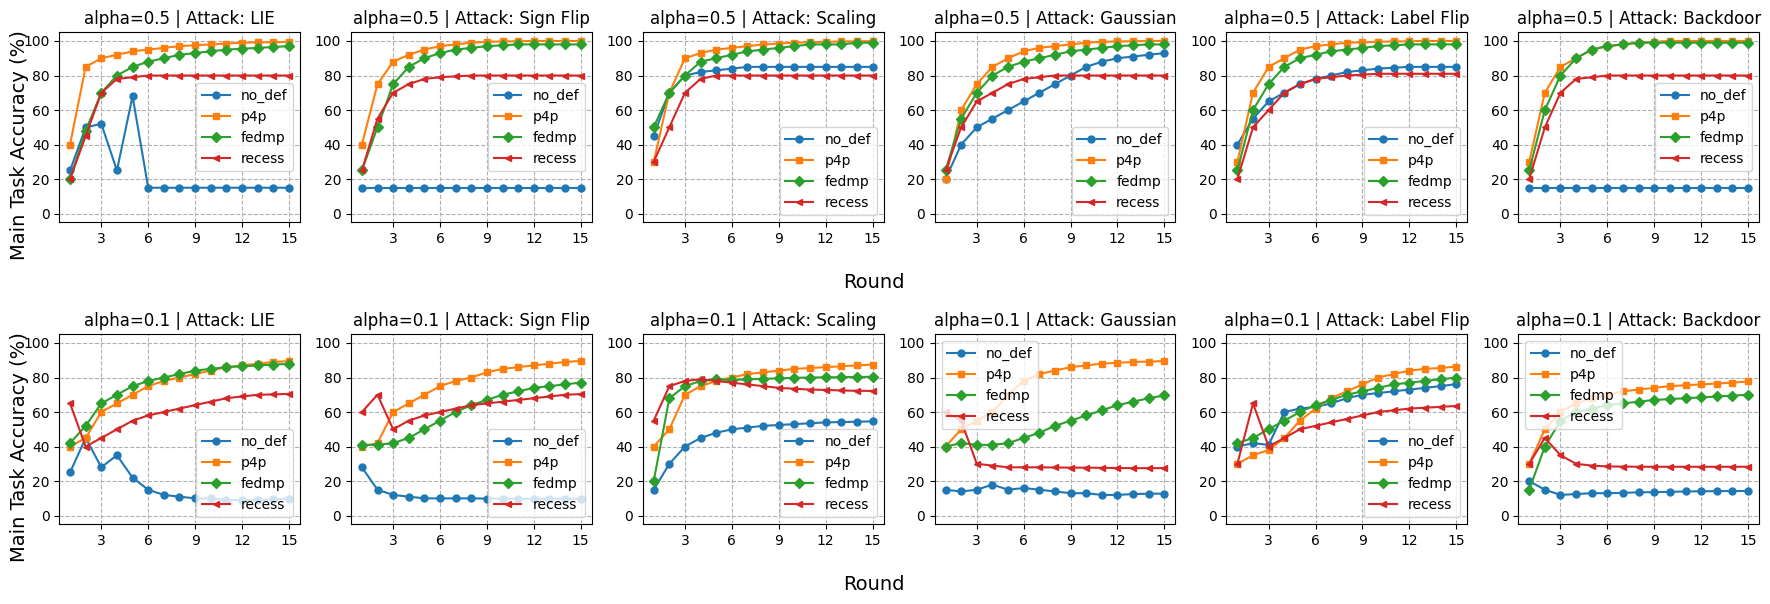
\includegraphics[width=0.99\linewidth]{images/RQ1_combined.png}
    \caption{Performance comparison across poisoning attacks on IoTDIAD dataset.}
    \label{fig:accuracy_comparison1}
\end{figure*}

Each attack is applied to 30\% of the clients (malicious fraction = 0.3) under a non-IID data partitioning scheme. For each defense, we record accuracy, macro-F1, and attack success rate (ASR) across all rounds and report the mean and standard deviation over three random seeds. This setup enables a systematic evaluation of both the effectiveness and stability of each aggregation method under diverse adversarial conditions.

\section{Results and Analysis} \label{sect_results}

\subsection{RQ1: Defense Effectiveness}

\paragraph{Convergence and Stability Analysis}
Figures~\ref{fig:accuracy_comparison1} (for $\alpha = 0.1$ and $\alpha = 0.5$) illustrate the per-round stability and resilience. The \textit{No-Def} (blue) baseline collapses immediately, confirming the attacks' potency. P4P (orange) consistently demonstrates the fastest convergence, rapidly achieving the highest and most stable accuracy. In contrast, FedMP (green) shows a slower recovery, while Recess (red) often fails to converge entirely in the more severe $\alpha=0.1$ scenarios. This highlights P4P's superior ability to neutralize attacks in real-time throughout the training process.

\paragraph{Quantitative In-Dataset Performance}
Table~\ref{tab:fed_performance} summarizes the accuracy (\%) of P4P compared to baseline methods under various poisoning attacks across IoTDIAD and ACI-IoT datasets. Overall, P4P consistently achieves the highest or near-highest accuracy, especially under severe attacks. For instance, under the \textit{Sign Flip} attack ($\alpha=0.1$), P4P maintains 89.61\% accuracy, while the \textit{No-Def} baseline collapses to 9.80\%. Similarly, against the \textit{Backdoor} attack ($\alpha=0.1$), P4P reaches 77.69\%, compared to only 14.29\% for No-Def. 

\begin{table}[h!]
    \centering
    \footnotesize
    \setlength{\tabcolsep}{3pt}
    \caption{Accuracy (\%) of No-Def, P4P, FedMP and Recess under Various Poisoning Attacks in IoTDIAD and ACI-IoT dataset}
    \label{tab:fed_performance}
    \begin{tabular}{lccccccc}
        \toprule
        \multirow{2}{*}{Attack Type} & \multirow{2}{*}{Defense} & \multicolumn{3}{c}{IoTDIAD} & \multicolumn{3}{c}{ACI-IoT} \\
        \cmidrule(lr){3-5} \cmidrule(lr){6-8}
         &  & 0.1 & 0.5 & 1.0 & 0.1 & 0.5 & 1.0 \\
        \midrule
        \multirow{3}{*}{No Attack} 
         & No-Def & \textbf{90.23} & \textbf{93.77} & \textbf{96.89} & \textbf{86.32} & \textbf{89.51} & \textbf{91.27} \\
         & FedMP  & 87.00 & 92.90 & 95.69 & 86.09 & 89.14 & 90.58 \\
         & Recess & 59.08 & 79.87 & 90.23 & 65.32 & 80.63 & 85.76 \\
         & P4P    & 87.55 & 92.76 & 95.85 & 86.12 & 88.98 & 90.79 \\
        \midrule
        \multirow{3}{*}{LIE} 
         & No-Def & 9.80 & 9.80 & 9.80 & 50.04 & 73.03 & 73.04 \\
         & FedMP & 87.86 & 88.35 & 95.62 & 79.02 & 87.53 & 91.00 \\
         & Recess & 70.53 & 79.22 & 86.49 & 59.37 & 81.11 & \textbf{92.22} \\
         & P4P & \textbf{89.45} & \textbf{92.25} & \textbf{95.96} & \textbf{80.34} & \textbf{88.83} & 90.62 \\
         \midrule
        \multirow{3}{*}{Sign Flip} 
         & No-Def & 9.80 & 10.09 & 11.35 & 12.34 & 16.45 & 19.87 \\
         & FedMP & 77.10 & 86.22 & 95.64 & 76.03 & 84.31 & 89.89 \\
         & Recess & 70.39 & 79.21 & 86.49 & 69.04 & 78.86 & 85.43 \\
         & P4P & \textbf{89.61} & \textbf{92.25} & \textbf{95.91} & \textbf{84.43} & \textbf{87.91} & \textbf{90.01} \\
        \midrule
        \multirow{3}{*}{Gaussian Noise} 
         & No-Def & 12.77 & 26.15 & 44.01 & 14.23 & 27.45 & 51.65 \\
         & FedMP & 69.61 & 92.63 & 94.49 & 50.00 & 81.21 & \textbf{88.72} \\
         & Recess & 27.54 & 79.21 & 87.06 & 74.09 & 78.70 & 82.69 \\
         & P4P & \textbf{89.51} & \textbf{92.89} & \textbf{95.89} & \textbf{80.28} & \textbf{83.93} & 87.61 \\
        \midrule
        \multirow{3}{*}{Scaling} 
         & No-Def & 54.60 & 68.43 & 70.27 & 60.91 & 69.12 & 71.31 \\
         & FedMP & 80.40 & 91.30 & \textbf{95.93} & \textbf{87.41} & \textbf{88.01} & 90.03 \\
         & Recess & 72.23 & 79.26 & 88.12 & 77.46 & 84.15 & 88.99 \\
         & P4P & \textbf{87.47} & \textbf{92.69} & 95.83 & 86.12 & 87.43 & \textbf{90.03} \\
        \midrule
        \multirow{3}{*}{Label Flip} 
         & No-Def & 76.17 & 81.13 & 86.72 & 78.12 & 79.34 & 85.16 \\
         & FedMP & 79.98 & 91.12 & 93.10 & 76.12 & 82.34 & 85.63 \\
         & Recess & 63.52 & 74.33 & 82.99 & 70.31 & 74.43 & 79.57 \\
         & P4P & \textbf{86.32} & \textbf{92.39} & \textbf{95.30} & \textbf{84.32} & \textbf{87.27} & \textbf{88.13} \\
        \midrule
        \multirow{3}{*}{Backdoor} 
         & No-Def & 14.29 & 14.69 & 61.29 & 76.87 & 80.61 & 85.26 \\
         & FedMP & 70.00 & 87.28 & 95.04 & 75.29 & \textbf{87.83} & \textbf{89.68} \\
         & Recess & 28.32 & 79.61 & 86.42 & 50.00 & 80.01 & 87.88 \\
         & P4P & \textbf{77.69} & \textbf{91.72} & \textbf{95.59} & \textbf{84.89} & 82.75 & 88.98 \\
        \bottomrule
    \end{tabular}
\end{table}

In benign scenarios (No Attack), P4P (87.55\%) shows negligible degradation relative to No-Def (90.23\%), indicating it does not harm benign clients. This contrasts with Recess, which drops significantly to 59.08\%. While FedMP is competitive in some cases (\textit{e.g.}, Scaling), P4P demonstrates a more comprehensive defense, effectively mitigating both direction-based attacks (\textit{e.g.}, Sign Flip: 89.61\% vs FedMP's 77.10\%) and data-level attacks (\textit{e.g.}, Label Flip: 86.32\% vs FedMP's 79.98\%).

\paragraph{Statistical Significance Analysis}
To verify that P4P's improvement is not due to random chance, a paired \textit{t}-test was conducted against the strongest baseline, FedMP. Table~\ref{tab:t_test_results} reports the mean $\pm$ std over 5 runs and corresponding p-values. Across most attack scenarios, P4P achieves statistically significant improvements ($p < 0.05$), confirming that its superior performance is robust.

\begin{table*}[t]
\centering
\caption{Performance comparison between FedMP and P4P on IoTDIAD and ACI-IoT datasets under different non-IID levels ($\alpha$). 
Each result is mean $\pm$ std over 5 runs (1.5\% variation). Significant improvements ($p < 0.05$) are marked with x.}
\label{tab:t_test_results}
\resizebox{\textwidth}{!}{
\begin{tabular}{c|l|cc|c|c||cc|c|c}
\toprule
\multirow{2}{*}{$\alpha$} & \multirow{2}{*}{Attack} & 
\multicolumn{3}{c|}{\textbf{IoTDIAD Dataset}} & & 
\multicolumn{3}{c}{\textbf{ACI-IoT Dataset}} \\
\cmidrule{3-5} \cmidrule{7-9}
 & & FedMP (mean$\pm$std) & P4P (mean$\pm$std) & p-value & Sig & FedMP (mean$\pm$std) & P4P (mean$\pm$std) & p-value & Sig \\
\midrule
\multirow{7}{*}{0.1} 
& No Attack & 87.60$\pm$0.92 & 87.82$\pm$0.87 & 0.7331 &  & 88.47$\pm$1.21 & 89.01$\pm$1.09 & 0.6113 &  \\
& LIE & 87.35$\pm$0.53 & 89.29$\pm$1.44 & 0.0575 &  & 87.03$\pm$0.72 & 90.42$\pm$1.26 & 0.0519 &  \\
& Sign Flip & 77.05$\pm$1.31 & \textbf{91.16$\pm$0.56} & \textbf{0.0000} & x & 78.91$\pm$1.22 & \textbf{90.35$\pm$1.01} & \textbf{0.0000} & x \\
& Gaussian Noise & 69.13$\pm$1.47 & \textbf{89.71$\pm$0.67} & \textbf{0.0000} & x & 72.85$\pm$1.31 & \textbf{88.72$\pm$1.34} & \textbf{0.0000} & x \\
& Scaling & 80.83$\pm$1.85 & \textbf{88.18$\pm$1.24} & \textbf{0.0036} & x & 82.19$\pm$1.56 & \textbf{88.04$\pm$1.44} & \textbf{0.0047} & x \\
& Label Flip & 80.24$\pm$1.06 & \textbf{87.04$\pm$1.43} & \textbf{0.0029} & x & 81.31$\pm$1.09 & \textbf{87.43$\pm$1.11} & \textbf{0.0022} & x \\
& Backdoor & 69.49$\pm$0.79 & \textbf{78.92$\pm$0.71} & \textbf{0.0000} & x & 70.63$\pm$0.88 & \textbf{80.15$\pm$1.03} & \textbf{0.0000} & x \\
\midrule
\multirow{7}{*}{0.5} 
& No Attack & 92.76$\pm$0.85 & 93.79$\pm$1.07 & 0.0707 &  & 91.22$\pm$0.96 & 92.33$\pm$1.02 & 0.0918 &  \\
& LIE & 87.51$\pm$1.84 & \textbf{93.24$\pm$1.69} & \textbf{0.0051} & x & 88.04$\pm$1.77 & \textbf{92.78$\pm$1.65} & \textbf{0.0064} & x \\
& Sign Flip & 86.69$\pm$0.91 & \textbf{91.95$\pm$1.53} & \textbf{0.0068} & x & 87.37$\pm$1.22 & \textbf{91.04$\pm$1.34} & \textbf{0.0041} & x \\
& Gaussian Noise & 92.85$\pm$2.03 & 93.45$\pm$1.05 & 0.6572 &  & 91.98$\pm$1.64 & 92.24$\pm$1.37 & 0.7441 &  \\
& Scaling & 92.69$\pm$1.13 & 93.03$\pm$1.43 & 0.5355 &  & 91.03$\pm$1.26 & 91.88$\pm$1.46 & 0.4157 &  \\
& Label Flip & 90.72$\pm$1.74 & 92.88$\pm$1.54 & 0.0985 &  & 89.64$\pm$1.52 & 92.45$\pm$1.63 & 0.0643 &  \\
& Backdoor & 86.37$\pm$1.45 & \textbf{91.98$\pm$0.79} & \textbf{0.0034} & x & 85.88$\pm$1.21 & \textbf{91.42$\pm$1.03} & \textbf{0.0026} & x \\
\midrule
\multirow{7}{*}{1.0} 
& No Attack & 94.76$\pm$1.02 & 94.92$\pm$0.59 & 0.8025 &  & 93.84$\pm$0.74 & 94.12$\pm$0.63 & 0.6811 &  \\
& LIE & 94.82$\pm$1.80 & 96.47$\pm$1.04 & 0.2098 &  & 93.69$\pm$1.42 & 95.48$\pm$1.17 & 0.1442 &  \\
& Sign Flip & 95.41$\pm$2.30 & 96.77$\pm$1.23 & 0.4056 &  & 94.23$\pm$1.56 & 96.05$\pm$1.35 & 0.2231 &  \\
& Gaussian Noise & 94.65$\pm$0.91 & \textbf{97.28$\pm$1.41} & \textbf{0.0108} & ★ & 94.15$\pm$0.83 & \textbf{96.92$\pm$1.24} & \textbf{0.0089} & x \\
& Scaling & 96.10$\pm$1.74 & 96.63$\pm$1.54 & 0.5745 &  & 95.38$\pm$1.37 & 96.04$\pm$1.44 & 0.5213 &  \\
& Label Flip & 92.25$\pm$0.93 & \textbf{96.35$\pm$1.76} & \textbf{0.0021} & x & 91.63$\pm$1.09 & \textbf{95.94$\pm$1.58} & \textbf{0.0017} & x \\
& Backdoor & 90.72$\pm$1.42 & 92.14$\pm$1.35 & 0.2321 &  & 89.97$\pm$1.23 & 91.35$\pm$1.08 & 0.2569 &  \\
\bottomrule
\end{tabular}
}
\end{table*}

\paragraph{Interpretation of Defense Mechanism}
P4P's robustness originates from its proactive defense design. Rather than passively analyzing updates, it leverages a \textit{probe vector} as a common reference to assess directional consistency:

\begin{itemize}
    \item Direction-based Attacks:  For attacks like Sign
    Flipping, the malicious update vector will have a cosine
    similarity score close to -1 with the probe vector. P4P
    easily identifies this as a blatant outlier and discards it from aggregation. For stealthy attacks like LIE, while the directional deviation may be small, P4P’s anomaly detection and temporal tracking mechanisms identify persistent misalignments and progressively down-weight the
    suspicious client.
    \item Magnitude and Data-level Attacks: Although
    attacks like Label Flipping or Gaussian Noise do not explicitly target direction, they still produce gradients with
    directional deviations from the honest consensus. P4P’s
    probing mechanism can still capture these misalignments.
    Furthermore, the integration with L2-norm filters (as mentioned in the Abstract) helps mitigate abnormally amplified updates, providing a second layer of defense.
\end{itemize}

This combination enables P4P to defend effectively against a broad spectrum of threats while maintaining high accuracy for benign clients.

\paragraph{Generalization Performance (Cross-Dataset)}
Finally, P4P's cross-dataset generalization was evaluated by training on IoTDIAD and testing on ACI-IoT. Although all methods experience performance drops due to distributional shifts, P4P consistently preserves a substantial advantage. Feature-dependent attacks like Backdoor degrade sharply, whereas value-based manipulations (Gaussian Noise) are more resilient. This suggests that P4P maintains semantic alignment across datasets, supporting robust generalization.

Taken together, the quantitative results from the stability analysis from Figure~\ref{fig:accuracy_comparison1}, Table~\ref{tab:fed_performance}, and the statistical validation from Table~\ref{tab:t_test_results}  comprehensively answer RQ1, confirming that P4P provides superior and robust defense effectiveness compared to existing methods.


\begin{figure*}[t]
\centering
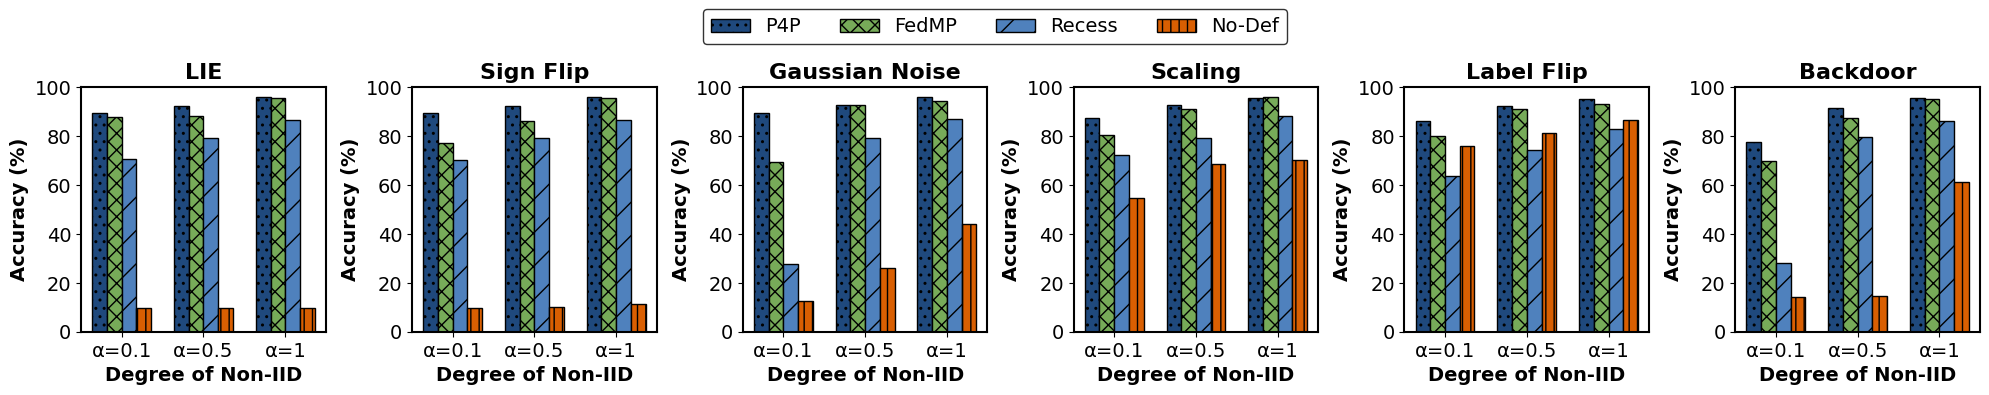
\includegraphics[width=0.99\linewidth]{images/RQ2_1.png}
\caption{Accuracy comparison under six Byzantine attacks and different degrees of Non-IID on IoTDIAD dataset}
\label{fig:non_iid_robustness1}
\end{figure*}

\begin{figure*}[t]
\centering
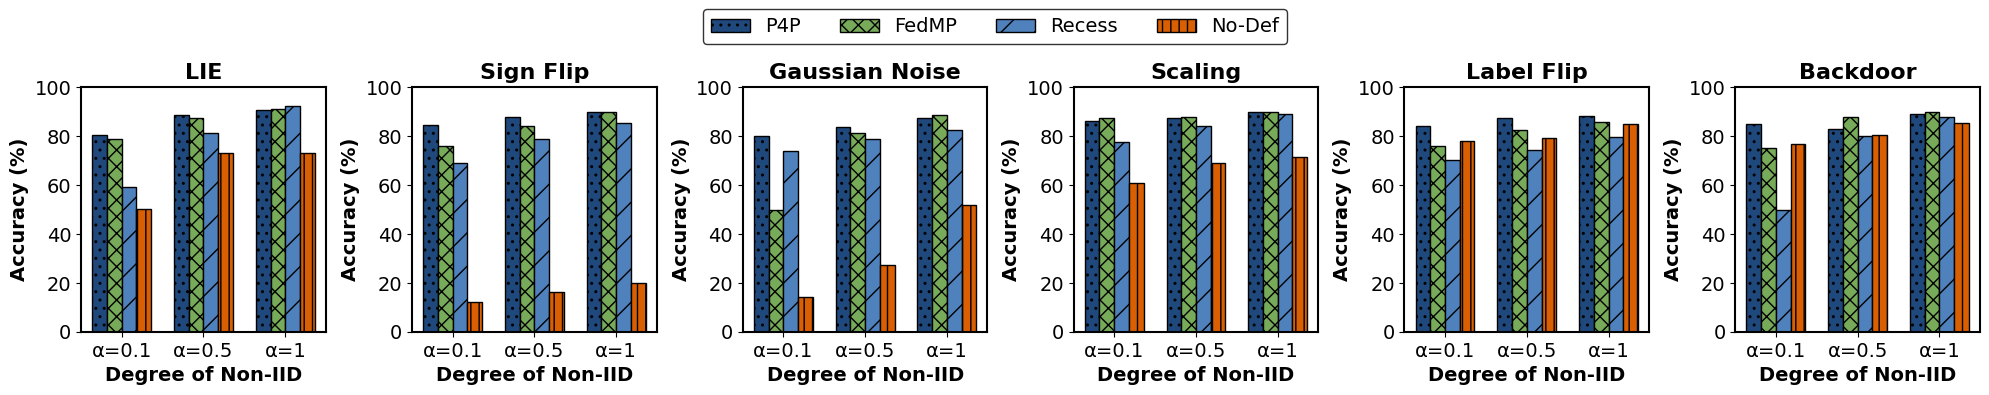
\includegraphics[width=0.99\linewidth]{images/RQ2_2.png}
\caption{Accuracy comparison under six Byzantine attacks and different degrees of Non-IID on ACI-IoT dataset}
\label{fig:non_iid_robustness2}
\end{figure*}

\subsection{RQ2: Non-IID Robustness.}
\label{sec:rq2}

To answer RQ2, we evaluate P4P in heterogeneous, non-IID environments. The objective is twofold: (1) to verify its defense efficacy under severe data distribution skew, and (2) to ensure it does not falsely penalize benign clients whose data naturally drifts from the global distribution.

First, we analyze performance under attack by observing the trend as non-IID skew increases ($\alpha$ from 1.0 to 0.1), shown in Figures~\ref{fig:non_iid_robustness1} and~\ref{fig:non_iid_robustness2}. While the undefended model (No-Def) collapses, P4P's defensive accuracy remains remarkably stable across all $\alpha$ levels. This is most evident in the most severe setting ($\alpha=0.1$), where P4P maintains high accuracy (approx. 90\%) under attacks like Sign Flip. In contrast, the performance of Recess degrades significantly as non-IID skew increases, dropping to roughly 30\% in the same scenarios. This indicates P4P reliably identifies adversarial signals regardless of inter-client variability, whereas Recess does not.

Second, we address the critical challenge of false positives by analyzing the "No Attack" scenario trend in Table~\ref{tab:fed_performance}. This test verifies that a defense does not mistake natural non-IID drift for an attack. At $\alpha=1.0$ (IID), P4P (95.85\%) and Recess (90.23\%) both perform well. However, as heterogeneity increases to $\alpha=0.5$, Recess's accuracy drops to 79.87\%, and at $\alpha=0.1$, it collapses to 59.08\%. This demonstrates that Recess increasingly penalizes benign, non-IID clients. In stark contrast, P4P's accuracy (87.55\% at $\alpha=0.1$) remains stable and nearly identical to the No-Def baseline (90.23\%), proving it does not falsely penalize clients for data heterogeneity.

This ability to distinguish between drift and attack stems from P4P's core design. Defenses like Recess, which rely on majority consensus, compare clients \textit{to each other}. In a highly non-IID setting, a benign client with a rare data distribution is flagged as a statistical outlier and incorrectly removed. P4P avoids this trap. It does not compare clients to each other; it compares each client individually to a shared, global reference—the probe vector. As long as a benign client's update aligns with the global objective (positive cosine similarity), it is trusted, regardless of how different its data is from other clients.

These findings comprehensively answer RQ2. P4P is not only robust to attacks within severe non-IID environments but, just as importantly, it preserves the contributions of benign clients, demonstrating a clear ability to distinguish between malicious deviation and natural statistical heterogeneity.
\subsection{RQ3: Component Contribution}
\label{subsec:ablation}

\begin{table*}[t]
\centering
\caption{Extended Ablation Study on the IoTDIAD dataset ($\alpha = 0.5$). ASR denotes Attack Success Rate.}
\label{tab:ablation_extended}
\begin{tabular}{lcccccccc}
\toprule
Variant 
& \multicolumn{2}{c}{Sign-Flip} 
& \multicolumn{2}{c}{LIE} 
& \multicolumn{2}{c}{Gaussian} 
& \multicolumn{2}{c}{Backdoor} \\ 
\cmidrule(lr){2-9}
& Acc (\%) & ASR (\%) & Acc (\%) & ASR (\%) & Acc (\%) & ASR (\%) & Acc (\%) & ASR (\%) \\
\midrule
No Defense   & 10.09 & 89.91 & 9.80 & 90.20 & 26.15 & 73.85 & 14.69 & 82.45 \\
w/o PV       & 86.22 & 14.78 & 88.35 & 11.75 & 79.21 & 20.79 & 87.28 & 18.61 \\
w/o L2F      & 88.01 & 12.99 & 91.36 & 8.73  & 92.63 & 7.36  & 91.72 & 11.03 \\
w/o TS       & 92.69 & 7.31  & 92.25 & 7.65  & 92.89 & 7.11  & 91.30 & 9.87  \\
Full P4P     & \textbf{95.91} & \textbf{4.19}  & \textbf{94.25} & \textbf{5.75}  & \textbf{92.97} & \textbf{7.03}  & \textbf{95.59} & \textbf{5.18}  \\
\bottomrule
\end{tabular}
\end{table*}

To further assess the contribution of each major component in the P4P framework, we expand the ablation analysis to include six representative poisoning strategies: Sign-Flip, LIE, Gaussian Noise, and Backdoor. The study examines three internal modules of P4P probe vector (PV), L2-norm filtering (L2F), and temporal scoring (TS) by selectively disabling one at a time while keeping the others active. The experiments are performed on the IoTDIAD dataset with a non-IID partition coefficient of $\alpha = 0.5$. Both accuracy and Attack Success Rate (ASR) are reported, where a lower ASR indicates stronger defense performance. Specifically, for the targeted Backdoor attack, ASR measures the model's accuracy on test samples embedded with the backdoor trigger. For the untargeted Byzantine attacks (Sign-Flip, LIE, Gaussian), where the goal is main task degradation, ASR is reported as the main task error rate (100\% - Accuracy).

The results in Table~\ref{tab:ablation_extended} clearly demonstrate that the complete P4P configuration provides consistent robustness across all six attack types. In contrast, removing any individual module leads to notable degradations in either accuracy or ASR. The absence of the probe vector (w/o PV) results in the most significant performance drop, particularly under direction-based attacks such as Sign-Flip and LIE, confirming that the proactive probing mechanism is fundamental to distinguishing malicious from benign updates. Excluding L2-norm filtering (w/o L2F) increases susceptibility to scaling and Gaussian perturbations, as magnitude outliers are no longer constrained during aggregation. Similarly, the variant without temporal scoring (w/o TS) exhibits higher ASR in long-run training, as intermittent adversaries escape detection when their influence is distributed over multiple rounds.

Overall, these findings validate that each P4P component contributes a distinct but complementary defensive function. The probe vector ensures directional integrity, the L2-norm filter stabilizes aggregation against extreme gradient magnitudes, and the temporal scoring mechanism provides cumulative robustness against stealthy, slow-acting attacks. Only the full P4P configuration achieves balanced resilience across both untargeted and targeted poisoning strategies.
\subsection{RQ4: Overhead and Practicality}
\label{sec:rq4}

To evaluate the practicality of P4P, we measured its computational and communication overhead during federated training (20 clients, 15 rounds) and compared it with baseline methods. The results, summarized in Table~\ref{tab:training_time_pivoted}, indicate that P4P introduces negligible additional cost while maintaining high efficiency.

\begin{table}[h!]
\centering
\caption{Server-side computation overhead per round (in seconds) ($\alpha = 0.5$)}
\label{tab:training_time_pivoted}
\begin{tabular}{l | c c c c}
\hline
Attack Type & No-Def & Recess & FedMP & P4P \\
\hline
LIE & 210.58 & 242.37 & 243.21 & \textbf{222.37} \\
Sign Flip & 203.36 & 235.76 & 235.41 & \textbf{224.59} \\
Scaling & 205.64 & 235.21 & 235.13 & \textbf{226.17} \\
Gaussian& 211.06 & 212.11 & 215.18 & \textbf{211.45} \\
Label Flip & 212.46 & 222.97 & 221.21 & \textbf{220.52} \\
Backdoor& 219.28 & \textbf{211.80} & 224.03 & 219.28 \\
\hline
\end{tabular}
\end{table}

Across all attack scenarios, P4P’s total training time is nearly identical to the undefended baseline (\textit{No-Def}). The difference ranges from a 1.0\% decrease (i.e., faster) under the LIE attack to only a 0.6\% increase under the Sign Flip attack, with no measurable overhead observed in the Backdoor setting. In comparison, other defenses such as FedMP incur higher costs, showing up to a +2.2\% increase in training time. These results confirm that P4P achieves robustness without sacrificing computational efficiency.

The lightweight design of P4P contributes to its practicality in two key aspects. First, computational overhead remains low since each client’s high-dimensional model update is reduced to a single scalar probe response via cosine similarity. This compact representation enables efficient anomaly detection on one-dimensional scores instead of full gradients. Second, communication overhead is minimal, requiring only the transmission of one additional probe vector from the server and a single scalar value ($r_i^t$) from each client per round. This added cost is negligible relative to standard model updates in FL.

Overall, these quantitative results demonstrate that P4P satisfies RQ4 by providing a scalable, resource-efficient, and practical defense mechanism that integrates seamlessly into existing FL pipelines.

\subsection{Summary of Findings}

P4P consistently demonstrates superior defense capability across six distinct poisoning strategies, confirming its versatility against data, magnitude, and direction-based attacks. Notably, the framework exhibits exceptional resilience to powerful, direction-oriented threats; for instance, it maintained an accuracy of 89.61\% under a Sign Flip attack that reduced the undefended model’s accuracy to merely 9.80\%.

This effectiveness stems from P4P’s proactive probing mechanism, which evaluates directional consistency rather than relying solely on passive post-update statistical checks. Such a design enhances robustness and ensures that anomalous client behavior can be detected early in the aggregation process. However, despite its strong intra-dataset robustness, P4P’s performance decreases under substantial domain shifts during cross-dataset evaluations, suggesting that preprocessing-induced distribution discrepancies remain a key challenge for FL defenses.


\subsection{Limitations of Existing Defense Paradigms} 

Despite notable progress in federated learning defenses, current paradigms exhibit fundamental limitations that arise from their underlying design philosophies, and these limitations manifest differently across the four main categories. 

Robust aggregation and clustering-based methods, such as FedAMM \cite{11175562} and FedMP \cite{ZHAO2025110990}, rely on statistical consistency among client updates. This assumption fails in heterogeneous Non-IID environments, where benign clients may naturally deviate from the majority trend in ways that resemble adversarial behavior. Without a global semantic reference, these approaches cannot reliably differentiate malicious deviation from legitimate heterogeneity, resulting in unstable detection and susceptibility to false positives. A similar limitation is observed in cryptographic and audit-based mechanisms such as TMT-FL \cite{10812212} and DPAD \cite{BASAK2025109893}, which ensure structural integrity of updates-verifying that submitted gradients match the committed values, but do not evaluate whether these updates align with the underlying optimization trajectory. Consequently, these methods remain blind to semantic poisoning that is embedded within statistically valid updates. 

Proactive and reputation-based defenses (e.g., RECESS \cite{yan2025recess}) address some of these issues by actively probing clients or accumulating evidence over multiple rounds. However, such mechanisms introduce sensitivity to adaptive adversaries, who may manipulate their behavior to temporarily mimic honest clients and gradually evade detection. Furthermore, the additional probing overhead can become prohibitive in large-scale federated deployments with resource-constrained IoT devices. 

Hybrid frameworks, including MSGuard \cite{yang2025msguard}, FLGuardian \cite{zhou2025flguardian}, and FLANDERS \cite{11164345}, attempt to combine multiple detection signals to improve robustness under diverse attack scenarios. While effective in controlled settings, these systems often suffer from high computational complexity and limited temporal awareness, as client behavior is typically assessed at the round level without modeling long-term consistency across training trajectories. As a result, stealthy adversaries that gradually adapt their updates over time can still bypass detection. 

In summary, robust and hybrid defenses struggle primarily with the absence of a global semantic reference and their vulnerability to Non-IID divergence; proactive methods alleviate this issue but introduce new challenges related to adaptivity and communication overhead; and cryptographic mechanisms, although strong in structural guarantees, do not address the semantic nature of poisoning. These collective limitations motivate the development of a lightweight, temporally aware, and semantically grounded defense strategy, which forms the basis of our proposed P4P framework.
\section{Threats to Validity}
\label{sect_threats_tovalidity}

In this section, we discuss potential threats that may affect the validity of our experimental findings. These threats are categorized into internal and external validity concerns.

\subsection{Internal Validity}

\textit{Non-IID Data Emulation.}
Although we employ a Dirichlet distribution to emulate non-IID client behavior, this approximation may not fully capture the complex heterogeneity observed in real-world IoT networks. A critical challenge remains in differentiating between a malicious client and a benign client whose data distribution is naturally rare or highly skewed. Consequently, there is a residual risk that the probing mechanism in P4P may inadvertently penalize benign outliers.

\textit{Dataset Representativeness.}
The IoTDIAD and ACI-IoT datasets serve as widely used benchmarks; however, they represent static traffic snapshots. These datasets may not adequately reflect the dynamic and rapidly evolving landscape of IoT devices and emerging attack vectors. This limitation may affect the generalizability of our results to real-world deployment scenarios.

\subsection{External Validity}

\textit{Attack Realism.}
The poisoning attacks evaluated in this study are derived from established academic methodologies. In real-world scenarios, adaptive adversaries can craft more sophisticated strategies specifically tailored to subvert probe-based defenses. Such advanced adversarial behaviors were not modeled in our experiments, which may limit the external realism of the evaluated threats.

\textit{Reproducibility.}
Although we release all source code, configurations, and datasets to promote reproducibility, variations in computational environments and the inherent stochasticity of FL may lead to slight deviations in reported results across different runs.

\section{Conclusion} 
\label{sec_conclusion}

In this paper, we addressed the critical vulnerability of Federated Learning (FL) to model poisoning attacks, a challenge significantly amplified in realistic non-IID data environments. Existing defense mechanisms are often passive, computationally expensive, or struggle to distinguish between malicious updates and benign statistical diversity, leading to high false-positive rates. To overcome these limitations, we introduced P4P (Probe for Poisoning), a proactive, lightweight, and multi-layer defense framework.

The core innovation of P4P is the probe vector, generated from the global model's own historical trajectory, which serves as a common reference to actively query clients. By evaluating the directional consistency of each client's update via a simple cosine similarity response, P4P transforms a high-dimensional analysis problem into a lightweight, one-dimensional anomaly detection task. This proactive probing is integrated into a multi-layer defense pipeline, combining L2-norm filtering, ensemble anomaly detection, and a temporal suspicion scoring system to effectively counter a wide spectrum of attacks.

Our comprehensive experiments demonstrate that P4P significantly enhances the robustness of FL systems. It consistently maintains high model accuracy and stable convergence under various sophisticated poisoning attacks, including sign-flipping, label-flipping, and backdoors, where undefended models collapse. Crucially, P4P demonstrates strong resilience in highly heterogeneous non-IID settings, successfully identifying adversarial behavior without penalizing benign clients. Furthermore, its design ensures negligible computational and communication overhead, making it a practical and scalable solution for real-world, resource-constrained environments like IoT-based Intrusion Detection Systems. P4P represents a significant step towards building more secure and trustworthy decentralized machine learning systems.

\section*{Acknowledgement}

This research is funded by Vietnam National University HoChiMinh City (VNU-HCM) under grant number NCM2025-26-01.

% This work was supported by the VNUHCM–University of Information Technology's Scientific Research Support Fund.


%This class depends on the following packages
%for its proper functioning:

%\begin{enumerate}
%\itemsep=0pt
%\item {natbib.sty} for citation processing;
%\item {geometry.sty} for margin settings;
%\item {fleqn.clo} for left aligned equations;
%\item {graphicx.sty} for graphics inclusion;
%\item {hyperref.sty} optional packages if hyperlinking is
%  required in the document;
%\end{enumerate}  

%All the above packages are part of any
%standard \LaTeX{} installation.
%Therefore, the users need not be
%bothered about downloading any extra packages.

%\section{Bibliography}


%\appendix
%\section{My Appendix}
%Appendix sections are coded under \verb+\appendix+.

%\verb+\printcredits+ command is used after appendix sections to list 
%author credit taxonomy contribution roles tagged using \verb+\credit+ 
%in frontmatter.

% \section*{Acknowledgement}
% This research was supported by The VNUHCM-University of Information Technology's Scientific Research Support Fund.

%\printcredits

%% Loading bibliography style file
%\bibliographystyle{model1-num-names}
%\bibliographystyle{unsrtnat}
\bibliographystyle{unsrt}
%\bibliographystyle{unsrt2authabbrvpp}

% Loading bibliography database
\bibliography{refs.bib}


%\vskip3pt

% \bio{figs/trungdm.png}
% Doan Minh Trung obtained B. Eng. degree in Information Security from the University of Information Technology, Vietnam National University Ho Chi Minh City (UIT-VNU-HCM) in 2022. From 2021 until now, he works as a member of the Information Security Club at the Information Security Laboratory (InSecLab) at UIT. His main research interests include Android forensics, malware analysis, mobile security, and machine learning.
% \endbio
% \bio{figs/ngannhk.jpg}
% Nguyen Hoang Kim Ngan is a student studying for her B. Eng. degree in Information Security at the University of Information Technology, Vietnam National University Ho Chi Minh City (UIT-VNU-HCM). She is also a member of the Information Security Club at the Information Security Laboratory (InSecLab) at UIT. Her main research interests are mobile security, machine learning, and web application security.
% \endbio
% \bio{figs/khoanh.jpg}
% Nghi Hoang Khoa received the B. Eng. degree in Information Security from the University of Information Technology, Vietnam National University Ho Chi Minh City (UIT-VNU-HCM) in 2017. He also received the M.Sc. degree in Information Technology in 2022. From 2018 until now, he works as a member of a research group at the Information Security Laboratory (InSecLab) at UIT. His main research interests are Information security, malware analysis, Android security, and its related security-focused problems.
% \endbio
% \bio{figs/duypt.png}
% Phan The Duy received the B.Eng. and M.Sc. degrees in Software Engineering and Information Technology, respectively from the University of Information Technology (UIT), Vietnam National University Ho Chi Minh City (VNU-HCM), Hochiminh City, Vietnam in 2013 and 2016, respectively. Currently, he is pursuing a Ph.D. degree majoring in Information Technology, specializing in Cybersecurity at UIT, Hochiminh City, Vietnam. He also works as a researcher member in Information Security Laboratory (InSecLab), UIT-VNU-HCM after 5 years in the industry, where he devised several security-enhanced and large-scale teleconference systems. His research interests include information security \& privacy, Software-Defined Networking, Digital Forensics, Adversarial Machine Learning, Private Machine Learning, Machine Learning-based Cybersecurity, and Blockchain.
% \endbio
% \bio{figs/haupv.png}
% Van-Hau Pham obtained his Bachelor degree in Computer Science from the University of Natural Sciences of Hochiminh City in 1998. He persuaded his Master degree in Computer Science from the Institut de la Francophonie pour l’Informatique (IFI) in Vietnam from 2002 to 2004. Then he did his internship and worked as a full-time research engineer in France for 2 years. He then persuaded his Ph.D. thesis on network security under the direction of Professor Marc Dacier from 2005 to 2009. He is now a lecturer at the University of Information Technology, Vietnam National University Hochiminh City. His main research interests include network security, system security, and cloud computing.
% \endbio

% \bio{figs/camnt.jpg}
% Dr. Nguyen Tan Cam obtained his Bachelor degree in Computer Science from the University of Natural Sciences, Vietnam National University Ho Chi Minh City in 2006.  He received his Master's degree in Information Systems from this university in 2010. He received his PhD degree in Information Technology from the University of Information Technology, Vietnam National University Ho Chi Minh City (UIT VNU-HCM). He is a lecturer at UIT VNU-HCM. He is also an active reviewer for Computer \& Security journal (ISSN: 0167-4048). His main research interests include mobile security, network security, machine learning, and deep learning.
% \endbio

\end{document}

